\documentclass[12pt, a4paper]{article}
\usepackage{../../../myconfig} % Gọi file cấu hình từ ngoài gốc vào

% ==========================================
% BẮT ĐẦU NỘI DUNG TÀI LIỆU
% ==========================================
\begin{document}

% Truyền 3 tham số: {Nhãn cam} {Chữ to chính giữa} {Chữ ở góc phải Header}
\titlebox{Chủ đề: định kì}{Đề kiểm tra định kì lần 4}{Đề định kì}

\textit{\textbf{Phần I: Thí sinh trả lời từ câu 1 đến câu 12, mỗi câu thí sinh chỉ chọn một phương án}}

\vspace{0.5cm}

% --- CÂU 1 ---
\questionLinesManual{0}{1}{Cho hàm số \(f(x)\) liên tục trên \(\mathbb{R}\) và có bảng biến thiên như hình vẽ.

\begin{center}

\begin{tikzpicture}
   % Cấu hình bảng biến thiên: kích thước cột và khoảng cách
   \tkzTabInit[lgt=1.5, espcl=2.2]
      {$x$ / 1 ,$f'(x)$ / 3}
      {$-\infty$, $1$, $2$, $3$, $+\infty$}
      
   % Vẽ các mũi tên biến thiên và giá trị tương ứng
   \tkzTabVar{-/ $-\infty$, +/ $-1$, -/ $-2$, +/ $5$, -/ $-\infty$}
\end{tikzpicture}
\end{center}

Hỏi hàm số \(y = f(x)\) có mấy cực trị?}{%
    \begin{tasks}(4)
        \task 1
        \task 2
        \task 3
        \task 0
    \end{tasks}
}

% --- CÂU 2 ---
\questionLinesManual{0}{2}{Một người chia thời lượng (đơn vị: giây) thực hiện các cuộc gọi điện thoại của mình trong một tuần thành sáu nhóm và lập bảng tần số ghép nhóm như sau:

\begin{center}
\begin{tabular}{|c|c|c|c|c|c|c|}
\hline
Nhóm & \([0;40)\) & \([40;80)\) & \([80;120)\) & \([120;160)\) & \([160;200)\) & \([200;240)\) \\
\hline
Tần số & 11 & 10 & 6 & 8 & 4 & 1 \\
\hline
\end{tabular}
\end{center}

Tứ phân vị thứ ba \(Q_3\) (đơn vị: giây) của mẫu số liệu ghép nhóm trên bằng}{%
    \begin{tasks}(4)
        \task 130
        \task 140
        \task 135
        \task 145
    \end{tasks}
}

% --- CÂU 3 ---
\questionLinesManual{0}{3}{Cho hàm số \(y = \dfrac{ax+b}{cx+d}\) (\(ac \neq 0, ad-bc \neq 0\)) có đồ thị như hình bên. Đường tiệm cận đứng của đồ thị hàm số đã cho có phương trình là

\begin{center}
\begin{tikzpicture}[scale=0.8, >=stealth]
    
    \begin{scope}
        \clip (-6, -4) rectangle (5, 6);
        
        % Nhánh bên trái của tiệm cận đứng (x < -1)
        \draw[ultra thick, samples=100, domain=-6:-1.2] plot (\x, {(2*\x-1)/(\x+1)});
        
        % Nhánh bên phải của tiệm cận đứng (x > -1)
        \draw[ultra thick, samples=100, domain=-0.8:4.5] plot (\x, {(2*\x-1)/(\x+1)});
    \end{scope}

    % Vẽ trục tọa độ
    \draw[->] (-6, 0) -- (5, 0) node[below] {$x$};
    \draw[->] (0, -4) -- (0, 6) node[left] {$y$};
    \node[below left] at (0,0) {$O$};

    % Vẽ tiệm cận ngang y = 2
    \draw[dashed,] (-6, 2) -- (5, 2);
    \node[above right] at (0, 2) {$2$};

    % Vẽ tiệm cận đứng x = -1
    \draw[dashed] (-1, -4) -- (-1, 6);
    \node[below left] at (-1, 0) {$-1$};
\end{tikzpicture}
\end{center}
}{%
    \begin{tasks}(4)
        \task \(x = 2\)
        \task \(y = 2\)
        \task \(y = -1\)
        \task \(x = -1\)
    \end{tasks}
}

% --- CÂU 4 ---
\questionLinesManual{0}{4}{Trong mặt phẳng với hệ tọa độ \(Oxy\), diện tích \(S\) của hình phẳng giới hạn bởi đồ thị của hàm số \(y = 2x - 3\), trục hoành và hai đường thẳng \(x = 1, x = 2\) được xác định bằng công thức}{%
    \begin{tasks}(2)
        \task \(S = \displaystyle\int_{1}^{2} |2x - 3| dx\)
        \task \(S = \pi \displaystyle\int_{1}^{2} |2x - 3| dx\)
        \task \(S = \pi \displaystyle\int_{1}^{2} (2x - 3)^2 dx\)
        \task \(S = \left| \displaystyle\int_{1}^{2} (2x - 3) dx \right|\)
    \end{tasks}
}

% --- CÂU 5 ---
\questionLinesManual{0}{5}{Cho cấp số cộng \((u_n)\) có \(u_1 = 4\) và công sai \(d = -3\). Giá trị của \(u_5\) bằng}{%
    \begin{tasks}(4)
        \task \(-8\)
        \task \(16\)
        \task \(-11\)
        \task \(19\)
    \end{tasks}
}

% --- CÂU 6 ---
\questionLinesManual{0}{6}{Tập nghiệm của phương trình \(\sin x = 0\) là}{%
    \begin{tasks}(2)
        \task \(S = \{k\pi \mid k \in \mathbb{Z}\}\)
        \task \(S = \left\{\dfrac{\pi}{2} + k2\pi \mid k \in \mathbb{Z}\right\}\)
        \task \(S = \{k2\pi \mid k \in \mathbb{Z}\}\)
        \task \(S = \left\{\dfrac{\pi}{2} + k\pi \mid k \in \mathbb{Z}\right\}\)
    \end{tasks}
}

% --- CÂU 7 ---
\questionLinesManual{0}{7}{Nghiệm của phương trình \(\log_3(2x-1) = 2\) là}{%
    \begin{tasks}(4)
        \task \(x = \dfrac{5}{2}\)
        \task \(x = \dfrac{7}{2}\)
        \task \(x = 4\)
        \task \(x = 5\)
    \end{tasks}
}

% --- CÂU 8 ---
\questionLinesManual{0}{8}{Họ nguyên hàm của hàm số \(f(x) = x^2\) là}{%
    \begin{tasks}(4)
        \task \(2x^3 + C\)
        \task \(\dfrac{1}{2}x^3 + C\)
        \task \(\dfrac{1}{3}x^3 + C\)
        \task \(3x^3 + C\)
    \end{tasks}
}

% --- CÂU 9 ---
\questionLinesManual{0}{9}{Tập giá trị của hàm số \(y = \dfrac{x-1}{x+1}\) là}{%
    \begin{tasks}(4)
        \task \(\mathbb{R} \setminus \{1\}\)
        \task \((1; +\infty)\)
        \task \(\mathbb{R} \setminus \{-1\}\)
        \task \(\mathbb{R}\)
    \end{tasks}
}

% --- CÂU 10 ---
\questionLinesManual{0}{10}{Cho \(\displaystyle\int_{1}^{2} f(x) dx = 3\); \(\displaystyle\int_{2}^{5} f(x) dx = 4\). Tính \(I = \displaystyle\int_{1}^{5} \left[ f(x) - \dfrac{x}{2} \right] dx\)}{%
    \begin{tasks}(4)
        \task \(I = 1\)
        \task \(I = 7\)
        \task \(I = 5\)
        \task \(I = -1\)
    \end{tasks}
}

% --- CÂU 11 ---
\questionLinesManual{0}{11}{Biết \(I = \displaystyle\int_{1}^{2} \dfrac{1}{2x^2 + 5x + 3} dx = \ln \dfrac{a}{b}\) với \(a, b\) là các số lớn hơn 1, phân số \(\dfrac{a}{b}\) tối giản. Giá trị \(T = a + b\) bằng}{%
    \begin{tasks}(4)
        \task 28
        \task 29
        \task 12
        \task 10
    \end{tasks}
}

% --- CÂU 12 ---
\questionLinesManual{0}{12}{Gieo ngẫu nhiên một con xúc xắc cân đối và đồng chất. Tính xác suất số chấm xuất hiện nhỏ hơn 4, biết rằng con xúc xắc xuất hiện mặt lẻ.}{%
    \begin{tasks}(4)
        \task \(\dfrac{1}{6}\)
        \task \(\dfrac{5}{6}\)
        \task \(\dfrac{1}{36}\)
        \task \(\dfrac{2}{3}\)
    \end{tasks}
}

\textit{\textbf{Phần II: Thí sinh trả lời từ câu 13 đến câu 16; trong mỗi ý a), b), c), d) ở mỗi câu, thí sinh chọn đúng hoặc sai.}}

\vspace{0.3cm}
% --- CÂU 13 ---
\questionTrueFalse{0}{13}{Cho hàm số \(f(x) = x^3 - 48x - 8\).}{
    \textbf{a)} & Hàm số đã cho có đạo hàm là \(f'(x) = 3x^2 - 48\).
    & \textcolor{amberorange}{$\bigcirc$} & \textcolor{amberorange}{$\bigcirc$} \\ \hline
    
    \textbf{b)} & Phương trình \(f'(x) = 0\) có tập nghiệm là \(S = \{4\}\).
    & \textcolor{amberorange}{$\bigcirc$} & \textcolor{amberorange}{$\bigcirc$} \\ \hline
    
    \textbf{c)} & \(f(4) = 248\).
    & \textcolor{amberorange}{$\bigcirc$} & \textcolor{amberorange}{$\bigcirc$} \\ \hline
    
    \textbf{d)} & Giá trị lớn nhất của hàm số \(f(x)\) trên đoạn \([-5;5]\) bằng 248.
    & \textcolor{amberorange}{$\bigcirc$} & \textcolor{amberorange}{$\bigcirc$} \\
}

% --- CÂU 14 ---
\questionTrueFalse{0}{14}{Một phần mềm nhận dạng tin nhắn quảng cáo trên điện thoại bằng cách dựa theo từ khóa để đánh dấu một số tin nhắn được gửi đến. Qua một thời gian dài sử dụng, người ta thấy rằng trong số tất cả các tin nhắn gửi đến, có 10\% số tin nhắn bị đánh dấu. Trong số các tin nhắn bị đánh dấu, có 10\% số tin nhắn không phải là quảng cáo. Trong số các tin nhắn không bị đánh dấu, có 10\% số tin nhắn là quảng cáo. Chọn ngẫu nhiên một tin nhắn được gửi đến điện thoại.}{
    \textbf{a)} & Xác suất để tin nhắn đó không bị đánh dấu bằng 0,9.
    & \textcolor{amberorange}{$\bigcirc$} & \textcolor{amberorange}{$\bigcirc$} \\ \hline
    
    \textbf{b)} & Xác suất để tin nhắn đó không phải là quảng cáo, biết rằng nó không bị đánh dấu, bằng 0,8.
    & \textcolor{amberorange}{$\bigcirc$} & \textcolor{amberorange}{$\bigcirc$} \\ \hline
    
    \textbf{c)} & Xác suất để tin nhắn đó không phải là quảng cáo bằng 0,82.
    & \textcolor{amberorange}{$\bigcirc$} & \textcolor{amberorange}{$\bigcirc$} \\ \hline
    
    \textbf{d)} & Xác suất để tin nhắn đó không bị đánh dấu, biết rằng nó không phải là quảng cáo, lớn hơn 0,95.
    & \textcolor{amberorange}{$\bigcirc$} & \textcolor{amberorange}{$\bigcirc$} \\
}

% --- CÂU 15 ---
\questionTrueFalse{0}{15}{Tại thời điểm \(t = 0\), một chiếc xe đang chuyển động về một hướng với vận tốc ban đầu \(v_0 = 10\) (m/s), gia tốc của xe từ thời điểm đó được tính bằng công thức \(a(t) = -2t + 4\) (m/s\(^2\)). Sau thời điểm đó 3 giây, do gặp chướng ngại vật nên xe bắt đầu phanh gấp và chuyển động biến đổi đều với gia tốc mới \(a_m(t) = -6\) (m/s\(^2\)).}{
    \textbf{a)} & Sau khi phanh gấp, xe chuyển động chậm dần đều.
    & \textcolor{amberorange}{$\bigcirc$} & \textcolor{amberorange}{$\bigcirc$} \\ \hline
    
    \textbf{b)} & Vận tốc của xe luôn tăng trong khoảng thời gian 3 giây đầu tiên.
    & \textcolor{amberorange}{$\bigcirc$} & \textcolor{amberorange}{$\bigcirc$} \\ \hline
    
    \textbf{c)} & Vận tốc của xe tại thời điểm \(t = 3\) giây là 3 (m/s).
    & \textcolor{amberorange}{$\bigcirc$} & \textcolor{amberorange}{$\bigcirc$} \\ \hline
    
    \textbf{d)} & Quãng đường xe đi được từ thời điểm \(t = 0\) đến khi dừng hẳn là 92 m.
    & \textcolor{amberorange}{$\bigcirc$} & \textcolor{amberorange}{$\bigcirc$} \\
}

% --- CÂU 16 ---
\questionTrueFalse{0}{16}{Cận kề ngày Tết Nguyên Đán, bác Nghĩa muốn thiết kế một đèn lồng cao 40 cm để treo lớn ở hiên nhà. Mặt cắt ngang tại mọi độ cao vuông góc với trục thẳng đứng của đèn lồng luôn là một hình vuông (xem hình vẽ). Mặt đáy và đỉnh của đèn lồng là hình vuông có cạnh \(L_0 = 10\sqrt{2}\) cm. Mặt cắt ngang tại vị trí rộng nhất của đèn lồng là hình vuông (hình vuông có diện tích lớn nhất) có cạnh \(L_{max} = 14\sqrt{2}\) cm. Mặt cắt của đèn lồng theo mặt phẳng đứng chứa đường chéo đáy có dạng là hình phẳng giới hạn bởi hai đường cong Parabol đối xứng nhau qua trục thẳng đứng đi qua tâm đáy của đèn lồng. Một đường cong Parabol \(y = f(x)\) trong bốn đường cong để tạo ra khung đèn lồng được gắn trong hệ trục \(Oxy\) với trục \(Ox\) biểu diễn chiều cao của chiếc đèn lồng (đơn vị mỗi trục là 1 cm).
\begin{figure}[H]
    \centering
    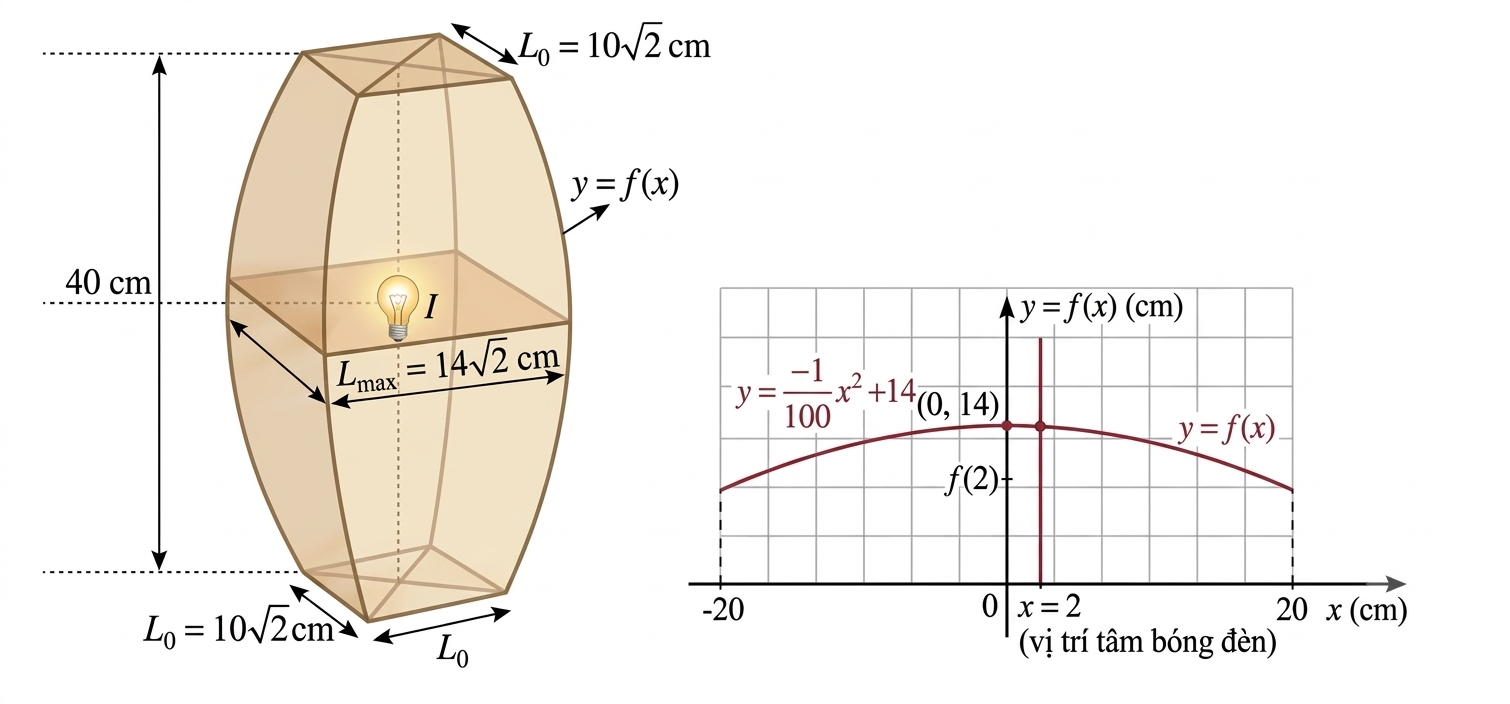
\includegraphics[width=0.7\textwidth]{images/Cau16.png}
\end{figure}
}{
    \textbf{a)} & Diện tích lớn nhất của một mặt cắt ngang hình vuông, vuông góc với trục thẳng đứng bằng 196 cm\(^2\).
    & \textcolor{amberorange}{$\bigcirc$} & \textcolor{amberorange}{$\bigcirc$} \\ \hline
    
    \textbf{b)} & Phương trình của đường cong Parabol \(y = f(x) = \dfrac{-1}{100}x^2 + 14\).
    & \textcolor{amberorange}{$\bigcirc$} & \textcolor{amberorange}{$\bigcirc$} \\ \hline
    
    \textbf{c)} & Thể tích của chiếc đèn lồng đó là 12,95 lít (làm tròn đến hàng phần trăm).
    & \textcolor{amberorange}{$\bigcirc$} & \textcolor{amberorange}{$\bigcirc$} \\ \hline
    
    \textbf{d)} & Để đảm bảo an toàn, bác Nghĩa treo một chiếc bóng đèn sợi đốt hình cầu có tâm (được xem là một điểm) đặt trên trục thẳng đứng của lồng đèn và cách đáy 22 cm. Bác quy định rằng để tránh làm cháy lớp giấy dán, khoảng cách từ mặt bóng đèn đến bất kỳ điểm nào trên lồng đèn phải ít nhất 7 cm. Bác có thể chọn chiếc bóng đèn có bán kính lớn nhất là 2,8666 cm (làm tròn đến bốn chữ số sau dấu phẩy).
    & \textcolor{amberorange}{$\bigcirc$} & \textcolor{amberorange}{$\bigcirc$} \\
}

\textit{\textbf{Phần III: Thí sinh trả lời từ câu 17 đến câu 22.}}

\vspace{0.3cm}
% --- CÂU 17 ---
\questionShortAnswer{0}{17}{Để gây quỹ từ thiện, câu lạc bộ thiện nguyện của một trường THPT tổ chức hoạt động bán hàng với hai mặt hàng là nước chanh và khoai chiên. Câu lạc bộ thiết kế hai thực đơn. Thực đơn 1 có giá 25 nghìn đồng, bao gồm hai cốc nước chanh và một túi khoai chiên. Thực đơn 2 có giá 40 nghìn đồng, bao gồm ba cốc nước chanh và hai túi khoai chiên. Biết rằng câu lạc bộ chỉ làm được không quá 165 cốc nước chanh và 100 túi khoai chiên. Số tiền lớn nhất mà câu lạc bộ có thể nhận được sau khi bán hết hàng bằng bao nhiêu nghìn đồng?
}

% --- CÂU 18 ---
\questionShortAnswer{0}{18}{Trên mặt phẳng vẽ hai nửa đường tròn đường kính \(AB, AD\), với \(AB = 2AD = 4\) cm như hình vẽ. Cho biết \(\widehat{BAC} = 30^\circ\). Hình phẳng \((H)\) là phần tô đậm nằm giữa hai nửa đường tròn, đường thẳng \(AB, AC\). Một kỹ sư cần chế tạo chi tiết máy bằng thép có dạng tròn xoay khi xoay hình phẳng \((H)\) quanh trục \(AB\). Biết chi phí sản xuất là 15 nghìn đồng/cm\(^3\). Giá tiền sản xuất một chi tiết máy là bao nhiêu nghìn đồng (kết quả làm tròn đến hàng đơn vị)?

\begin{center}
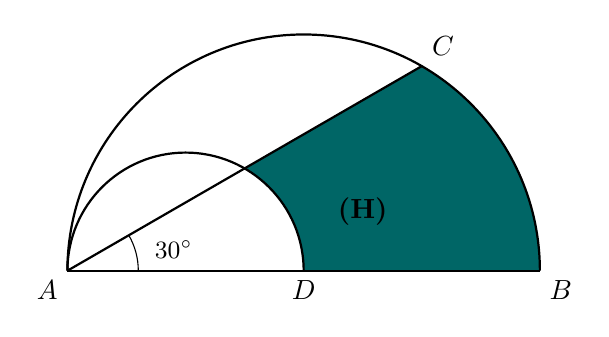
\begin{tikzpicture}[scale=1.5]
    % Đặt gốc A tại (0,0)
    % AB = 4cm => B = (4,0)
    % AD = 2cm => D = (2,0)
    % Nửa đường tròn lớn có tâm O1(2,0), bán kính R = 2
    % Nửa đường tròn nhỏ có tâm O2(1,0), bán kính r = 1
    % Tia AC tạo với AB góc 30 độ, C nằm trên đường tròn lớn: C = (2 + 2*cos 60°, 2*sin 60°) = (3, sqrt(3))
    % Giao điểm E của AC với nửa đường tròn nhỏ: E = (1 + 1*cos 60°, 1*sin 60°) = (1.5, sqrt(3)/2)

    % 1. Tô màu hình phẳng (H)
    % Biên gồm: Đoạn DB (từ 2 đến 4) -> Cung BC (tâm O1, R=2, góc 0° đến 60°) 
    %           -> Đoạn CE -> Cung ED (tâm O2, r=1, góc 60° về 0°) -> khép kín.
    \fill[teal!80!black] (2,0) -- (4,0) 
        arc [start angle=0, end angle=60, radius=2] 
        -- (1.5, {sqrt(3)/2}) 
        arc [start angle=60, end angle=0, radius=1] -- cycle;

    % Nhãn (H)
    \node at (2.5, 0.5) {\textbf{(H)}};

    % 2. Vẽ nửa đường tròn lớn (đường kính AB)
    \draw[thick] (4,0) arc [start angle=0, end angle=180, radius=2];

    % 3. Vẽ nửa đường tròn nhỏ (đường kính AD)
    \draw[thick] (2,0) arc [start angle=0, end angle=180, radius=1];

    % 4. Vẽ đường thẳng AB
    \draw[thick] (0,0) -- (4,0);

    % 5. Vẽ tia AC (đi qua E và C)
    \draw[thick] (0,0) -- (3, {sqrt(3)}) node[above right] {$C$};

    % 6. Ký hiệu góc 30 độ
    \draw (0.6,0) arc [start angle=0, end angle=30, radius=0.6];
    \node at (0.9, 0.18) {\small $30^\circ$};

    % 7. Đặt nhãn cho các điểm
    \node[below left] at (0,0) {$A$};
    \node[below] at (2,0) {$D$};
    \node[below right] at (4,0) {$B$};

\end{tikzpicture}
\end{center}
}

% --- CÂU 19 ---
\questionShortAnswer{0}{19}{Một khối bê tông có chiều cao 2 mét được đặt trên mặt đất. Nếu cắt khối bê tông bởi một mặt phẳng nằm ngang và cách mặt đất \(x\) mét (\(0 \leq x \leq 2\)) thì được mặt cắt là một hình chữ nhật có chiều dài 5 mét và chiều rộng bằng \((0,5)^x\) mét (xem hình dưới). Thể tích của khối bê tông đó bằng bao nhiêu mét khối (Kết quả làm tròn đến hàng phần mười)?
\begin{figure}[H]
    \centering
    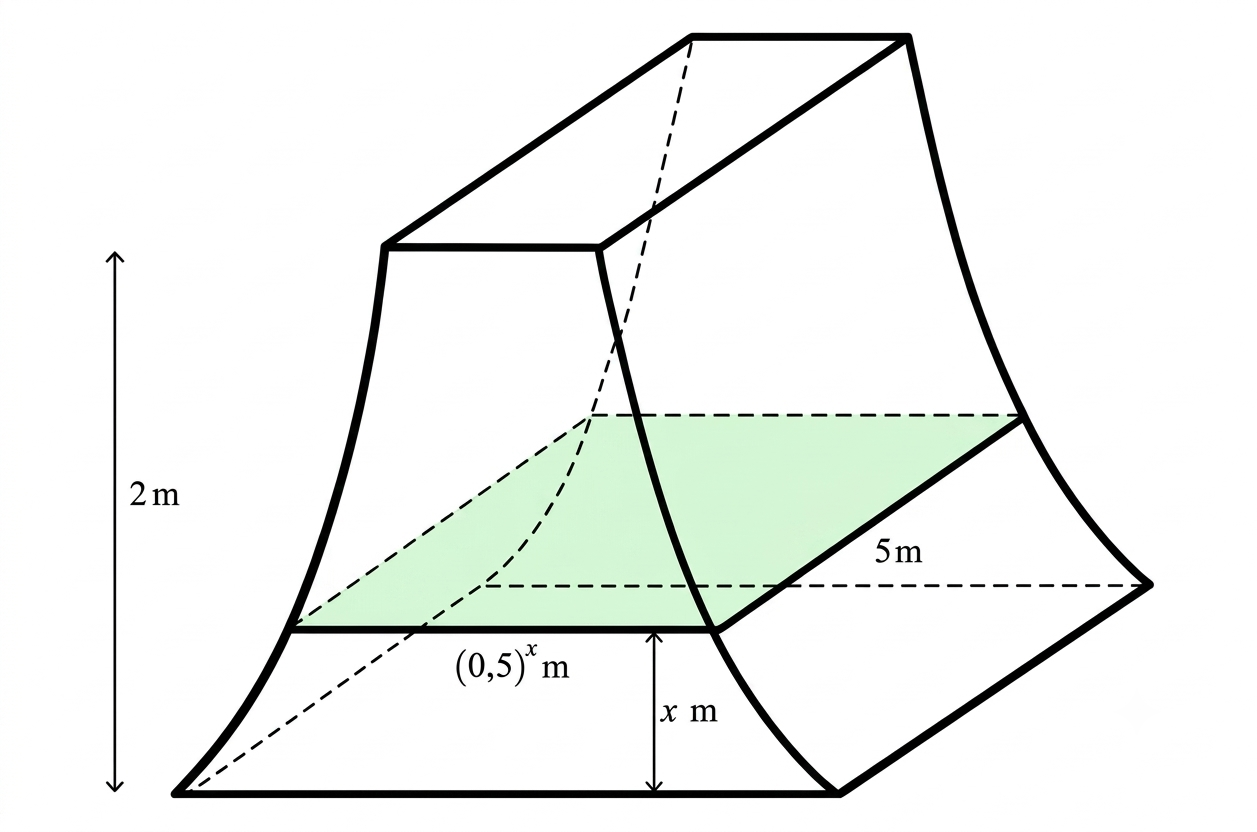
\includegraphics[width=0.5\textwidth]{images/Cau19.png}
\end{figure}
}

% --- CÂU 20 ---
\questionShortAnswer{0}{20}{Một bể bơi hình bán nguyệt có đường kính là \(AB = 100\) m. Một người muốn bơi từ vị trí \(A\) đến vị trí \(C\) theo phương thẳng rồi lên bờ đi bộ từ \(C\) đến \(B\). Biết rằng vận tốc bơi là 5 km/h và vận tốc đi bộ là 6 km/h. Hỏi thời gian tối đa để người đó hoàn thành lộ trình như trên là bao nhiêu phút? (Làm tròn kết quả đến hàng phần trăm).

\begin{center}
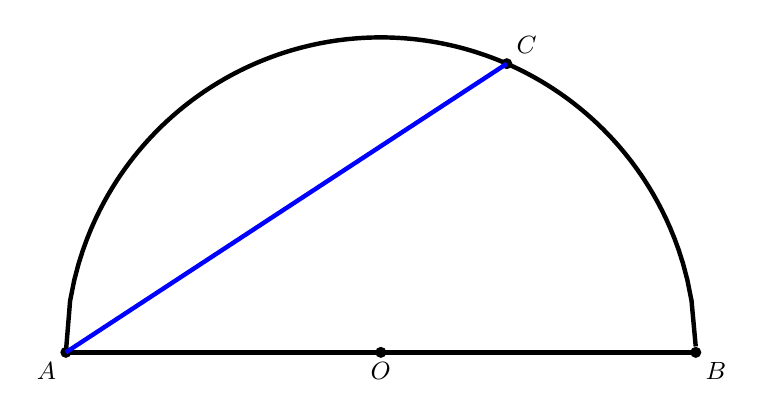
\begin{tikzpicture}[>=latex, scale=0.8]
    % 1. Vẽ bể bơi hình bán nguyệt
    \draw[ultra thick, samples=150, domain=-5:5, color=black] 
        plot (\x, {sqrt(25 - \x*\x)});
    \draw[ultra thick, black] (-5,0) -- (5,0);
    
    % 2. Đánh dấu các điểm
    \fill (-5,0) circle (2.5pt);
    \node[below left] at (-5,0) {\small $A$};
    
    \fill (5,0) circle (2.5pt);
    \node[below right] at (5,0) {\small $B$};
    
    \fill (0,0) circle (2.5pt);
    \node[below] at (0,0) {\small $O$};
    
    % 3. Đánh dấu điểm C trên bán nguyệt
    \fill (2,{sqrt(21)}) circle (2.5pt);
    \node[above right] at (2,{sqrt(21)}) {\small $C$};
    
    % 4. Vẽ đường bơi và đường đi bộ
    \draw[ultra thick, color=blue] (-5,0) -- (2,{sqrt(21)});
    
\end{tikzpicture}
\end{center}
}

% --- CÂU 21 ---
\questionShortAnswer{0}{21}{Một phần đường chạy của tàu lượng siêu tốc (Hình 1) khi gắn hệ trục tọa độ \(Oxy\) được mô phỏng ở Hình 2, đơn vị trên mỗi trục là mét.
\begin{figure}[H]
    \centering
    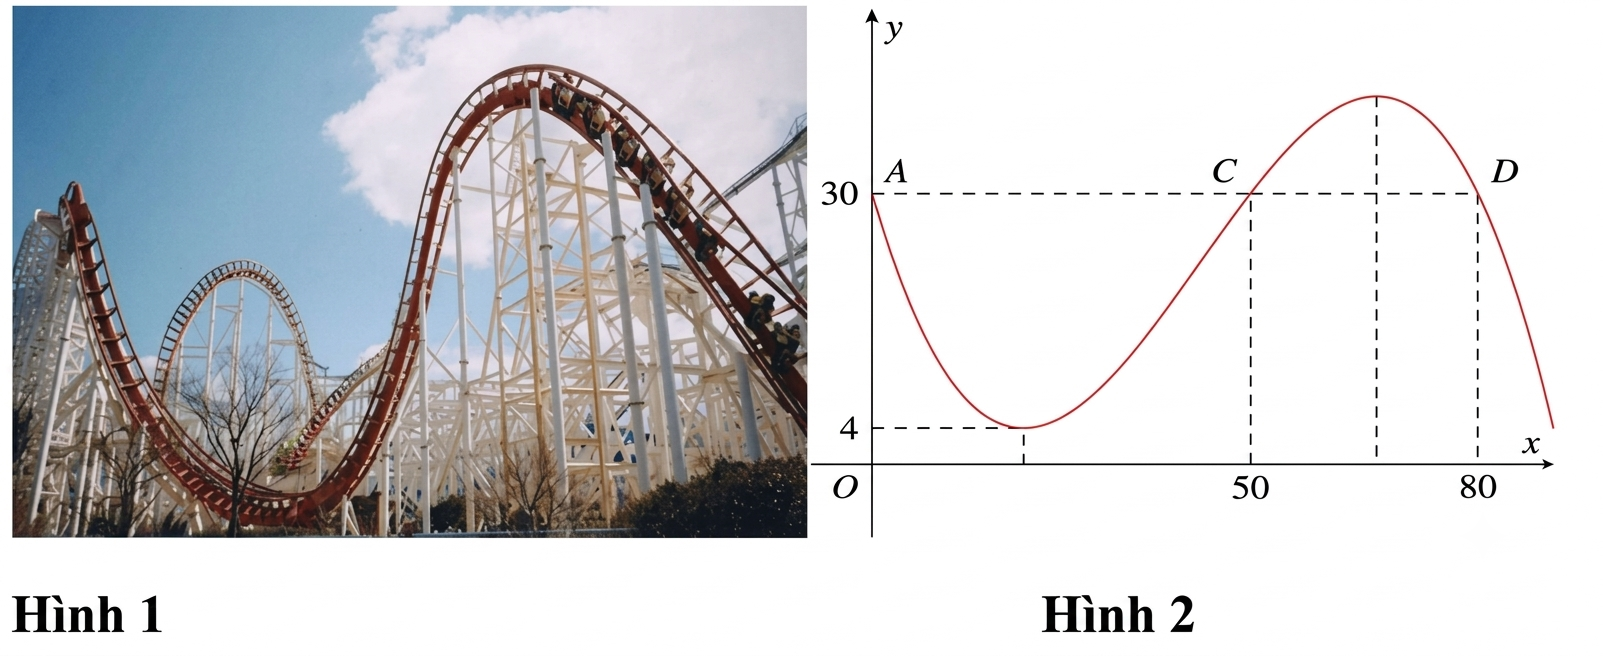
\includegraphics[width=0.7\textwidth]{images/Cau21.png}
\end{figure}

Biết đường chạy của nó là một phần đồ thị hàm số bậc ba \(y = ax^3 + bx^2 + cx + d\) (\(0 \leq x < 90\)); tàu lượn siêu tốc xuất phát từ điểm \(A\), đi qua các điểm \(C, D\) (ba điểm \(A, C, D\) nằm trên đường thẳng song song với trục \(Ox\)) đồng thời đạt độ cao nhỏ nhất so với mặt đất là 4 m. Độ cao lớn nhất mà tàu lượng siêu tốc đạt được là bao nhiêu mét so với mặt đất (kết quả làm tròn đến hàng phần chục)?
}

% --- CÂU 22 ---
\questionShortAnswer{0}{22}{Một máy ép thủy lực có hai động cơ \(A\) và \(B\) hoạt động độc lập với nhau. Xác suất để động cơ \(A\) chạy tốt là 0,8. Xác suất để động cơ \(B\) chạy tốt là 0,75. Biết rằng máy chỉ hoạt động được nếu có ít nhất một động cơ chạy tốt. Tìm xác suất để máy ép thủy lực hoạt động.
}

\end{document}

%1B,2C,3D,4A,5A,6A,7D,8C,9A,10A,11B,12D,13DSSS, 14DSDD, 15 DSSS, 16SDDD, 17:2150, 18:192, 19:5.4 , 20:1.65, 21:40.7, 22:0.95